\documentclass[12pt, a4pape]{article}
\usepackage[utf8]{inputenc}
\usepackage{fancyhdr}
\usepackage{caption}
\usepackage{multicol}
\usepackage[english, russian]{babel}
\usepackage{amsmath}
\usepackage{amssymb}
\usepackage{makecell} % Для выравнивания внутри ячйки
\usepackage{graphicx} % Вставка картинок правильная
\usepackage{float} % "Плавающие" картинки
\usepackage{wrapfig} % Обтекание фигур (таблиц, картинок и прочего)
\usepackage{array}
\usepackage{booktabs}

\usepackage{geometry}
\geometry{  
    a4paper,
    top=8mm, 
    right=16mm, 
    bottom=20mm, 
    left=8mm
}

\setlength{\columnsep}{29pt} % расстояние между колонками

\pagestyle{fancy}
\fancyhf{} % Очистка всех полей заголовков
\renewcommand{\headrulewidth}{0} % Убираем линию вверху страницы

% С этого момента начинается разные части для main.tex

\fancyfoot[R]{\Huge \thepage} % Номер страницы справо

\setcounter{page}{5} % Меняем номер страницы
\setcounter{figure}{2} % Меняем номер рисунков
\setcounter{table}{1} % Меняем номер таблиц

\usepackage[font=scriptsize, justification=raggedright, singlelinecheck=false]{caption}

\begin{document}
    \begin{figure}[ht]
        \centering
        % Первый график
        \begin{minipage}[t]{0.45\textwidth}
            \centering
            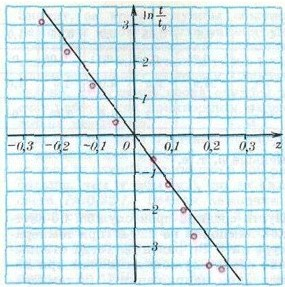
\includegraphics[width=\linewidth]{images/pict2.jpg}
            \caption{}
        \end{minipage}
        \hfill
        % Второй график
        \begin{minipage}[t]{0.45\textwidth}
            \centering
            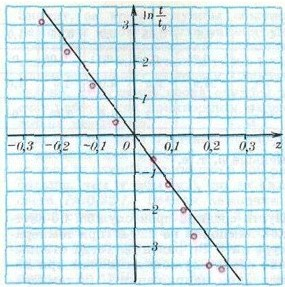
\includegraphics[width=\linewidth]{images/pict2.jpg}
            \caption{}
        \end{minipage}
    \end{figure}
    \begin{multicols}{2}
        \noindent 
        показана зависимость величины $y = \ln \frac{I}{I_0}$ от $z = 1 - \frac{U_0}{U}$ (необходимые данные приведены в той же таблице 2). Экспериментальные точки хорошо ложатся на прямую линию. Логарифмический масштаб по оси $y$ выбран потому, что если бы в формуле для $I(T)$ не было стоящего перед экспонентой множителя, то зависимость $y(T)$ имела бы вид: \[y = \ln \frac{I}{I_0} = \frac{T_{\text{кр}}}{T_0} \left(1 - \frac{T_0}{T}\right),\] величина же $\theta = 1 - \frac{T_0}{T},$ как можно заключить из данных таблицы 1, с хорошей точностью пропорциональна $z$ (чтобы догадаться до этого, нужны были некоторые наводящие соображения, связанные с балансом энергии в лампочке): $ \theta \approx Kz,$ где коэффи-

        \hfill {\raggedright \scriptsize Таблица 2}
        
        \noindent % Убираем отступ перед таблицей
        \setlength{\tabcolsep}{3pt} % Уменьшаем отступы между столбцами для равномерного заполнения
        \renewcommand{\arraystretch}{1.5} % Увеличиваем высоту строк для аккуратности
        \begin{tabular*}{\columnwidth}{|c@{\extracolsep{\fill}}|c|c|c|c|c|c|}
            \hline
            $U$, В & 220 & 120 & 130 & 150 & 180 & 190\\ \hline
            $U_0 / U$ & 1 & 1,81 & 1,66 & 1,47 & 1,14 & 1,12 \\ \hline
            $z$ & 0 & $-0,81$ & $-0,66$ & $-0,47$ & $-0,14$ & $-0,12$\\ \hline
            $r$, см & 27 & 5,5 & 8 & 13 & 21 & 22 \\ \hline
            $I / I_0$ & 1 & 0,05 & 0,09 & 0,23 & 0,60 & 0,66 \\ \hline
            $y$ & 0 & $-3,0$ & $-2,4$ & $-1,5$ & $-0,5$ & $-0,4$ \\ \hline
        \end{tabular*}
        \\
        
        \noindent
        -циент пропорциональности $K$ равен примерно $0,3$. Наличие множителя перед экспонентой вызывает отклонение зависимости $y(z)$ от строгой пропорциональности, однако эти отклонения невелики.\\

        \noindent \textbf{Почему лампочка перегорает?}\\
        
        \noindentПричина перегорания лампочки ясна — это испарение вольфрама. Для того чтобы от поверхности нити оторвалась молекула вольфрама, необходимо, чтобы кинетическая энергия её теплового движения $W \sim kT$ стала больше энергии связи молекулы с остальным кристаллом $w$. Согласно закону статистической физики, вероятность такого события пропорциональна $e^{-w/kT}$. Значит, число молекул, отрывающихся от нити в единицу времени,
        \[ n \sim e^{-w/kT}.\]
        
        \noindentВеличину $w$ можно определить из значения теплоты испарения вольфрама при комнатной температуре $Q \approx 850 \, \text{кДж/моль}$:
        \[ w = \frac{Q}{N_A} \approx \frac{1,4 \times 10^{-19} \, \text{Дж}}{\text{К}} \quad (\text{число Авогадро}),\]
        величина $k \cdot T$, имеющая размерность температуры, около $10^5 \, \text{К}$.
        
        Предположим, что нить перегорает после полного испарения определённого количества молекул. Это означает, что время службы лампочки тем больше, чем
        аоитваоивитовпититит
    \end{multicols} 



\end{document}